\normalfont\normalsize
\chapter{Software Implementation}

The entire solution is devided into different modules that run independently  but communicate with each other to achive the main purpose. The idea of software organized as modules allows for future features to be added more easily.

The main modules are installed in the AR Parrot Drone and the android FreeFlight 2.0 application.

The SparrowDongle gateway is always in a listen for data state and dumps every data received on the serial. When it receives the data, it sends back an ack to let the SparrowV3.2 node to know that it can begin sending the entire stored data to the mobile gateway. 

The SparrowV3.2 node is sending periodically a small data packet to check if a gateway is available. When it receives the ack for the packet it starts sending the stored data to the gateway. The data sent can vary, from sensor readings to debugging informations in order to check the state of the Wireless Sensor Network.

The data gathered by the gateway is saved into different files in the AR Parrot Drone's internal memory. The files also contains informations such as the node identification tag and time of the transfer. The data can be accessed at any time by any device connected to the drone's wireless network port 4242 via FTP.

The drone also process some collected data to provide informations like signal strength, last connection time and number of nodes. This informations are send to the controlling device through a socket connection.

The controling device, pc or android, will gather the informations and display them to the user.

\clearpage

\begin{figure}[ht]
\begin{center}
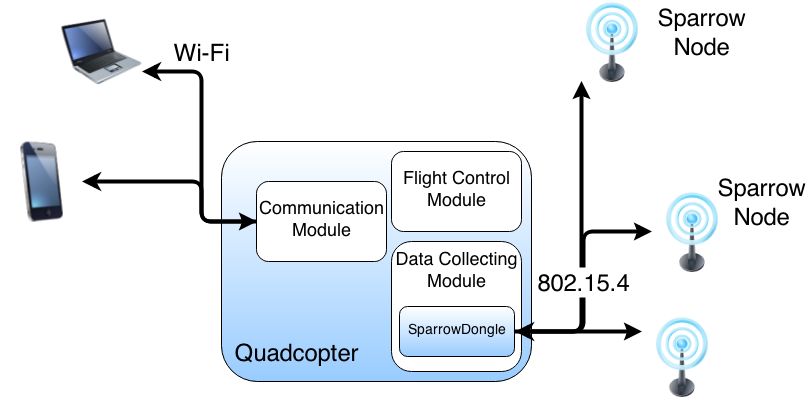
\includegraphics[width=0.9\textwidth]{implementation/organigrama.png}
\end{center}
\caption{\small \itshape{Modules and connections between them and devices}}
\end{figure}



\section{The Debug Module}

The code can be compiled to display debug informations to the console or to supress them entirely. Also, in certain parts of the modules, a wait action is need in order to wait for an action to be executed. Now the delay is set at 100 ms, but it can be easily modiffied to any desired value. 

\lstset{numbers=none, mathescape=true, nolol=false,caption=Data Collection use of mutex,label=lst:task}
\begin{lstlisting}
/* activates/deactivates printf debuf information*/
#define DEBUG_ON 0
/* delay yime in microseconds*/
#define DELAY_US 100000
#define DEBUG_PRINT(a...) { if(DEBUG_ON) printf(a); }
\end{lstlisting}

 

\section{The Data Collecting Module}
 
The module saves the collected data int-o the drones internal memory and pases the data in order to gather certain informations like number of nodes currently connected to the Dongle, de signal strength, if the Dongle is connected etc. This informations are passed to the communication module to provide to the user realtime feedback.

This module, besides the main purpose and similar to the other modules, has some extra features that are design to make the solution more user friendly and easier to improve in the feature.

\subsection{Modules intercommunication}

The memory area in which the informations sent to the user are saved is shared between this module and the comunication module. Basically, the way this two modules interract with each other can be compared to the consumer - producer problem, where the Data Collecting Module can be associated with the producer side and the Communication Module with the consumer side.

The main problem consists of deadlocks and data starvation. This is prevent with the use of one mutex that allows only one thread at a time to moddify the informations.

\lstset{numbers=none, mathescape=true, nolol=false,caption=Data Collection use of mutex,label=lst:task}
\begin{lstlisting}
pthread_mutex_lock(&data_lock); 
add_node_data(get_current_timestamp(),read_data + 7);
pthread_mutex_unlock(&data_lock);
\end{lstlisting}

The mutex is used similarly in the Communication Module when it consumes the information.


\subsection{Failure proof}

Because the Dongle is connected to an USB port on a machine that has a lot of vibrations, it might desconnect / reconnect for a very short period of time, so this module has been designed  with multiple USB disconnects and reconnects without the need to reset the Drone. This infomation is vital, because you can check if the Dongle is still connected to the dron without the need to inspect it visualy or to connect to a debug terminal.

\section{The Communication Module}

All the information gathered by the Data Collecting Module would be useless if it cannot be accesed easily. 

This module, as the name suggests, handles the communication of this this crucial information back to the user.

Being a different module, with different attributions than the Data Collecting Module, it has an entire proccess dedicated to it for 3 important reasons:
\begin{itemize}

\item 1. This approach of a module with its one procces allows the modules to run indepently of each other;
\item 2. The Data Collecting Module can collect the data from the Dongle as soon as as it has a new one available;
\item 3. If the Communication Module stops working, the Data Collecting Module continues to save the new informations received. 

\end{itemize}

\subsection{Socket with connection reset}

The communication is done through socket connections listening on port 8888. It accepts only one connection at a time.

If a connected client decides to disconnect before or while a write is performed, a SIGPIPE error signal will be thrown, stopping all the modules. This is prevent by ignoring the signal, forcing the write acction to return a EPIPE, an exiting the this function.

The main proccess will calback the accept\_socket\_connection to reestablish a new connetion. Once a connection is established, it will send information once every DELAY\_US microseconds. The program was configured and tested with a 100 ms wait period that leeds to a ten times per second information update.

This delay is required because:
\begin{itemize}

\item If data is send to often , the socket might be flooded and stop sending the data
\item If there were no delay, it will create an big and useless processor busy state both for the drone and the controlling device.

\end{itemize}

 
\subsection{JSON Encoding of Data}

The data sent is encoded in JSON format, because it is very easy to encode and all devices can decode it.

The informations ecoded are
\begin{itemize}

\item Dongle conection status
\item An array containing node informations
\begin{itemize}

	\item Node unique ID
	\item Last conection time of the node to Dongle
	\item The power of the received signal

	\end{itemize}
\end{itemize}


\section{Android application modules}

\begin{figure}[ht]
\begin{center}
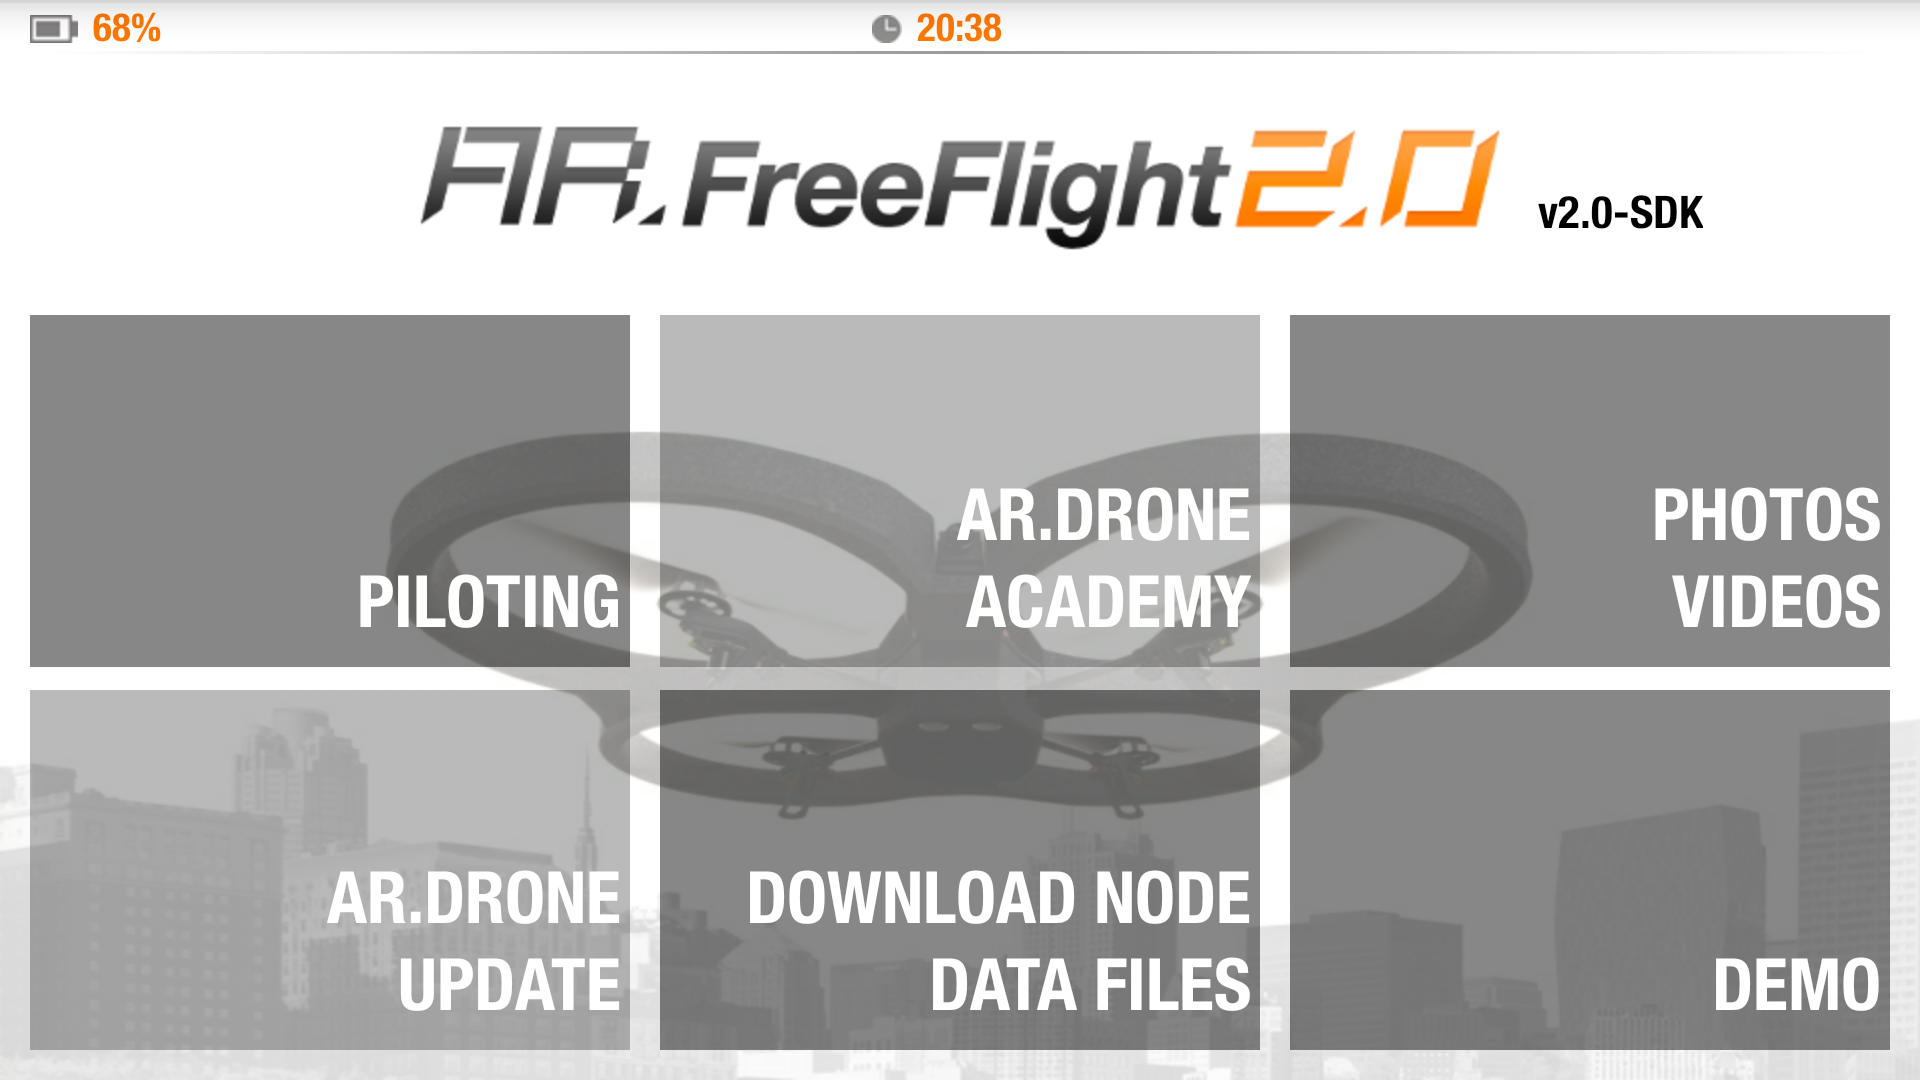
\includegraphics[width=0.9\textwidth]{implementation/android_app.png}
\end{center}
\caption{\small \itshape{ARFreeflight modified application}}
\end{figure}

Being an opensource platform we have moddified the AR Freeflight 2.0 android application to communication with our new modules added tot the drone.

Android fairly imposes the use of the background process class AsynkTask when you have to use communication protocols like http, ftp, sockets. This prevents the ui process from being stuck in communication and not responding to user actions. 

The class offers 5 very important methods that can be overwritten, 3 running on the main ui process, that prepare data before and after exection, publish  the progress or simply cancel at any step, and 1 running on the actual background process.


\subsection{Display information module}

\begin{figure}[ht]
\begin{center}
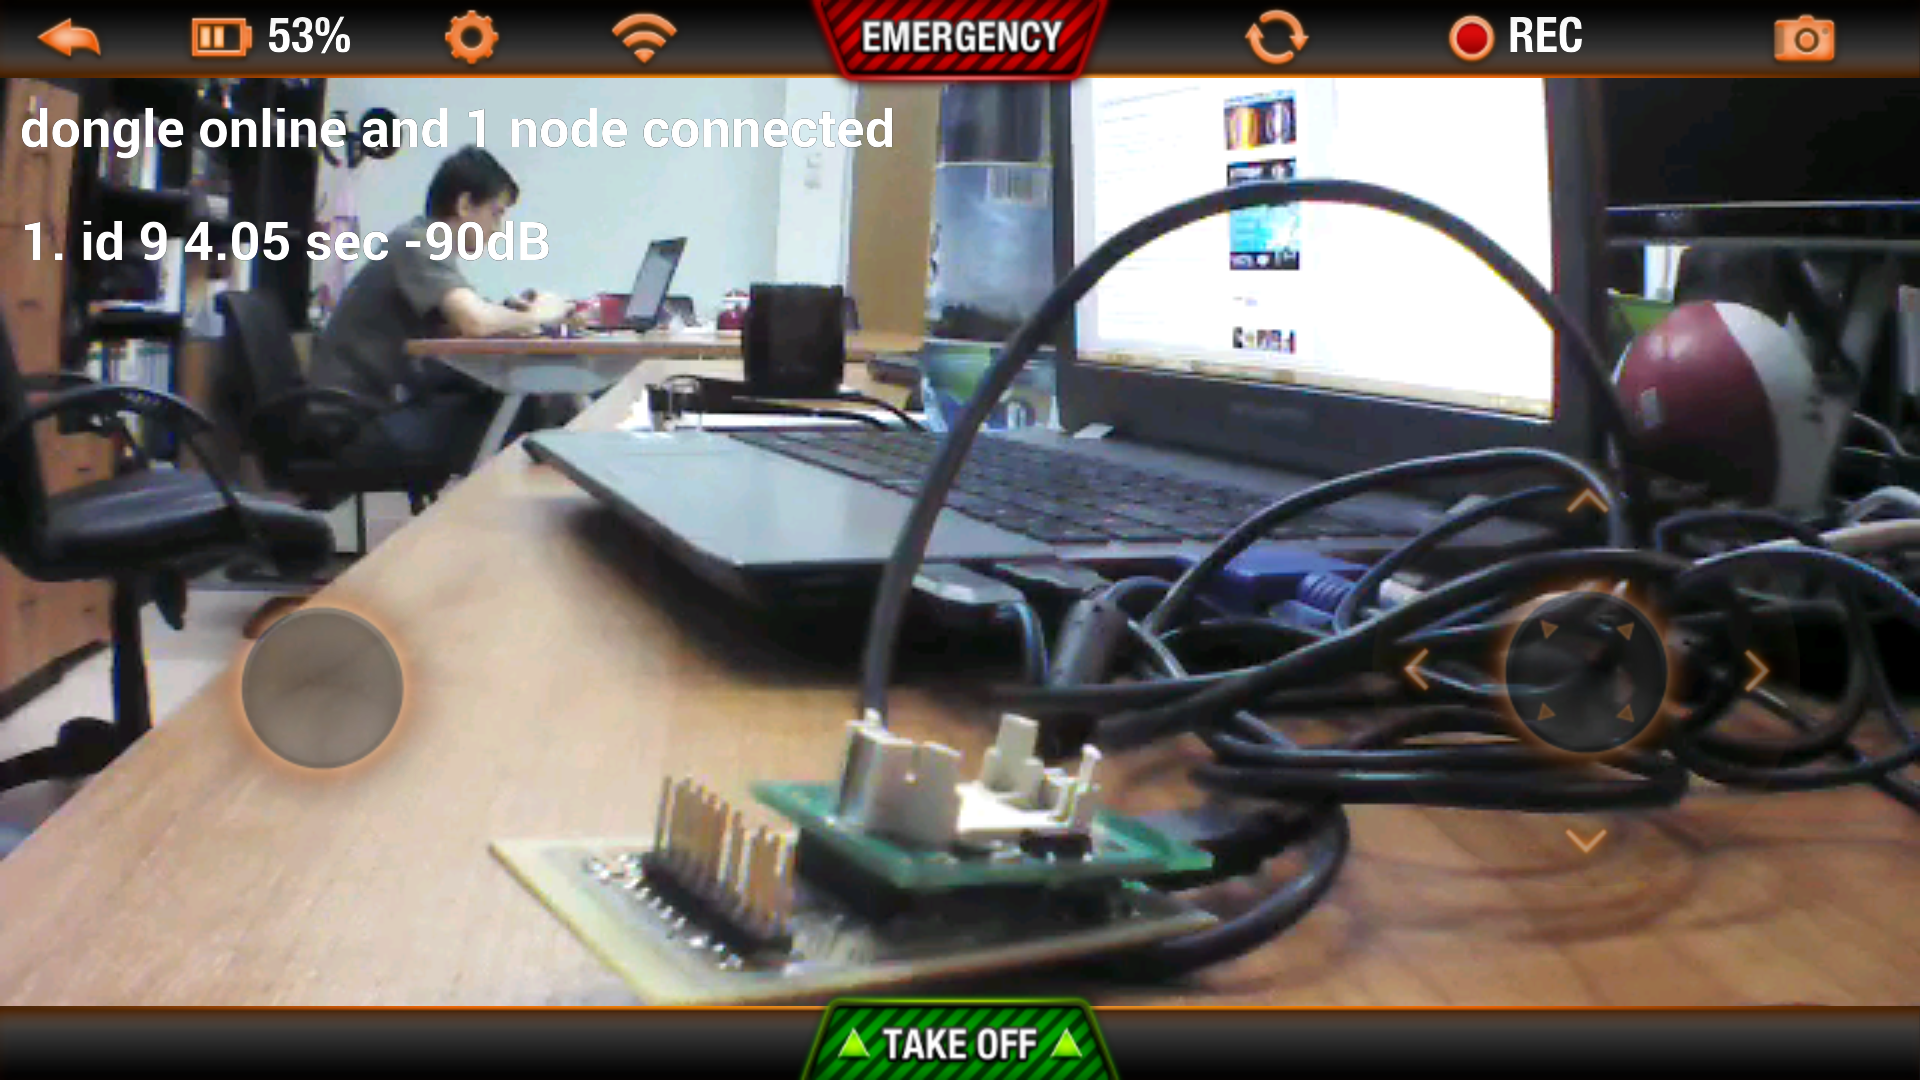
\includegraphics[width=0.9\textwidth]{implementation/android_info.png}
\end{center}
\caption{\small \itshape{ARFreeflight modified Piloting Screen}}
\end{figure}

The Piloting screen of the application has been modified to the display the received informations from the drone. 

The information displayed consists of the dongle being functional and at most, 9 nodes sorted descending after their signal strength. 
  
\subsection{FTP communication module}

\begin{figure}[ht]
\begin{center}W
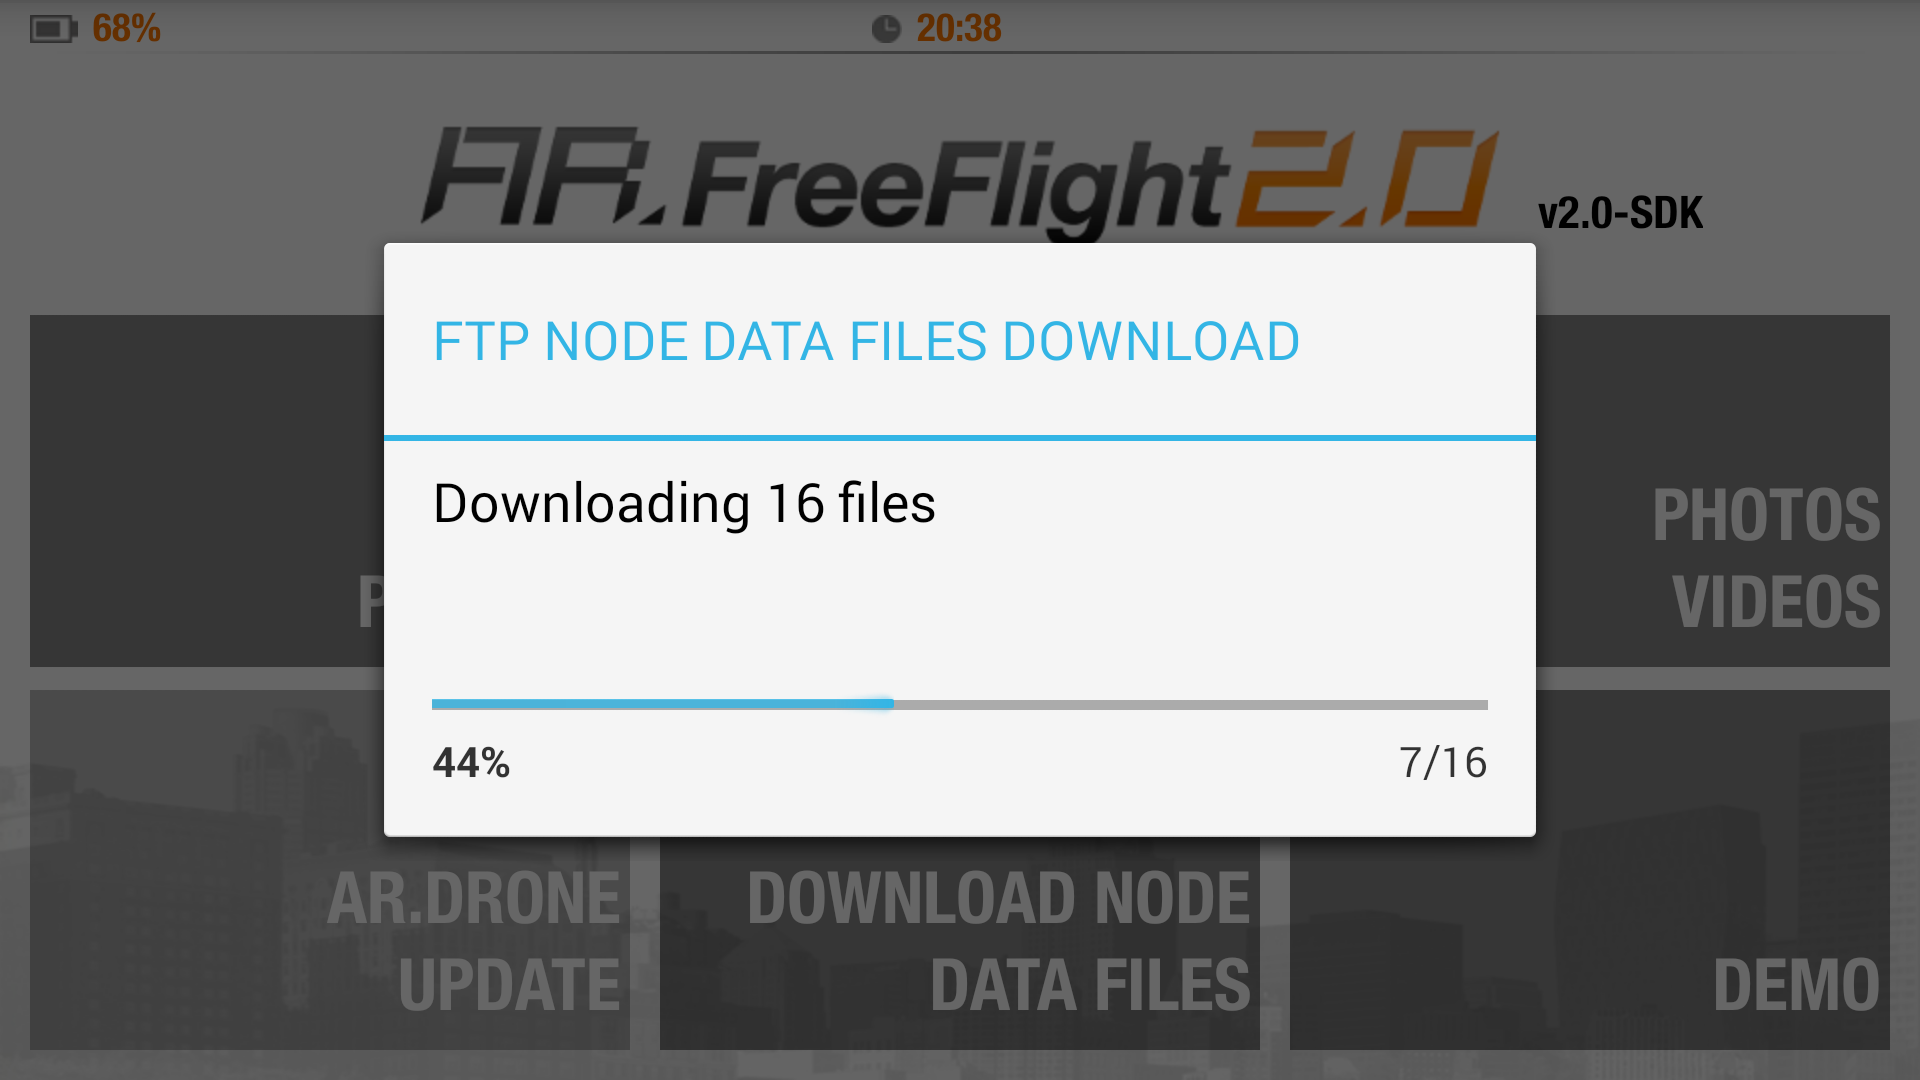
\includegraphics[width=0.9\textwidth]{implementation/android_ftp.png}
\end{center}
\caption{\small \itshape{ARFreeflight FTP downloading files}}
\end{figure}

The drone has a build in FTP server that can be configured to allow acces to any folders/files on the drone. We have configured the drone so that the folder that contains the saved data can be accesed at any time using the 4242 port by any device that has FTP client capabilities. We have added this feature to the android application as well.

The application will download all the files from the drone to the local storage of your android device while displaying the progress.
 

